\documentclass[12pt]{article}
\usepackage[T1]{fontenc}
\usepackage{graphicx}
\usepackage{caption}
\usepackage{array}
\title{Systemy Wbudowane\\
   Projekt\\
   Schemat komponentów i połączeń}
\author{Piotr Popis}
\date{Maj 2020}

\begin{document}

\begin{titlepage}
\maketitle
\end{titlepage}

\section{Schemat Połączeń}
\subsection{Schemat w kontekście fizycznym}
\subsubsection{Obwód}
\hspace{-2.75cm}%                
    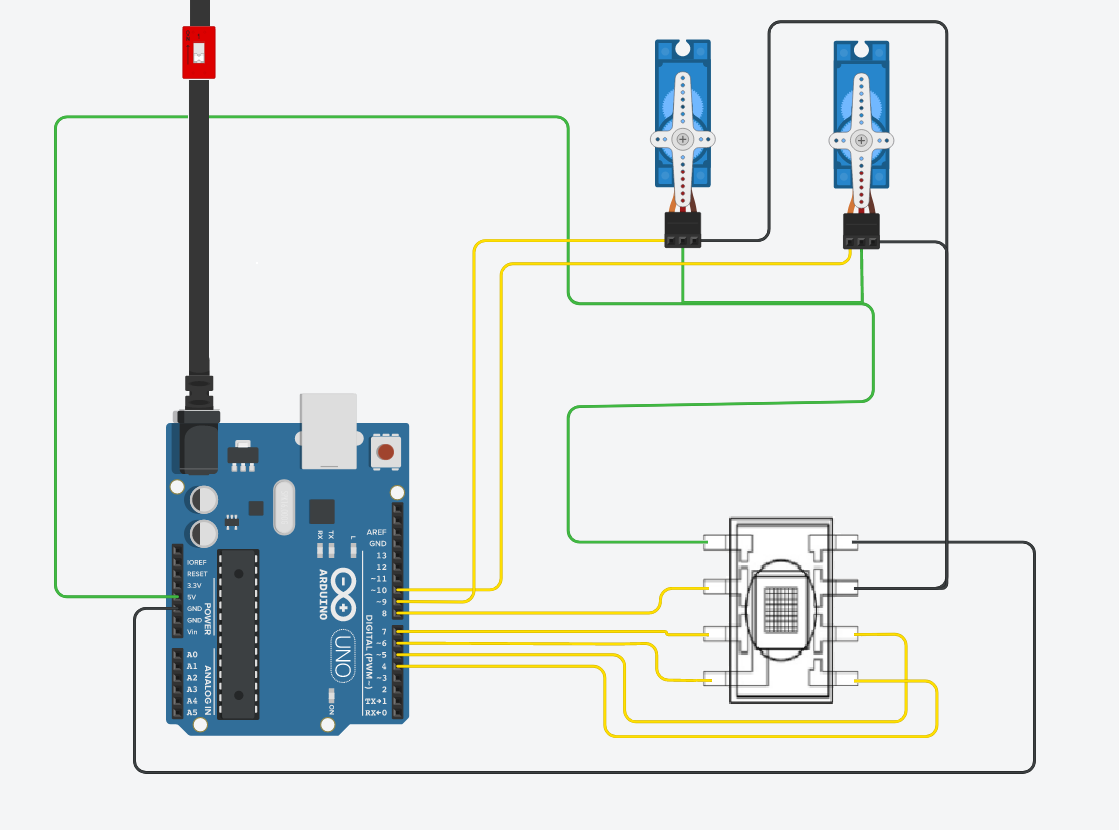
\includegraphics[scale=0.5]{circuit_better.png}
Wszystkie linie( połączenia) to copper wires. 
\newpage
\subsubsection{Opis Obwodu}
Gniazdo GND płytki Arduino Uno R3 jest połączone z gniazdem GND na sensorze TCS 3200. "Ziemia" (Power supply Ground) krzyżuje się z drugim wire również łączącym GND obu serw z OE(Enable for output frequency) sensora. Napięcie 5V poprowadzone jest zielonym wire'm do serwa górnego, dolnego oraz sensora TCS pod gniazdem VCC w każdym z komponentów. Gniazdo PWM  serwa górnego i dolnego podłączone jest do pinów cyfrowych 10 i 9 na płycie Arduino. Gniazdo OUT sensora, z którego zczytywana jest częstotliwość(frequency output) połączone jest w pinie 8 z płytką AUR3. Gniazda S2,S3(Photodiode type selection inputs) sensora, na które wysyłane są sygnały przez płytkę HIGH,LOW w celu określenia natężeń RGB( tabela 1.1.2) z pinami 6,5 płytki arduino. I ostatnie połączenia kablowe to S1,S0 wejścia selekcji, skalowania częstotliwości wyjściowej połączone z pinem 4, 5 w płytce Arduino.
\subsection{Schemat Interakcji}
\subsubsection{Opis}
\begin{enumerate}

\item Arduino przesyła do serwa górnego żądanie z kątem przesunięcia. \item Serwo górne odbiera sygnał i przenosi obiekt pod sensor TCS.\item  Arduino wysyła kolejno sygnały (High,High) ; (Low,High) ; (Low,Low)  przez wejścia S2,S3 do sensora TCS. Krócej: arduino pyta sensor TCS o kolor obiektu. \item TCS zwraca( OUT) częstotliowść zwrotną dla zadanej kombinacji. TCS zwraca odpowiedź na zapytanie o kolor do Arduino.\item  Arduino wysyła do serwa dolnego kąt pod jakim ma się ustawić. \item Serwo dolne ustawia zsuw pod odpowienim kątem z wiadomości od Arduino. \item Arduino wysyła sygnał do serwa górnego. \item Serwo góne przesuwa się zgodnie z rozkazem. \item Arduino ustawia serwo górne do stanu zerowego.\item  Wszystko się zapętla aż do wyłączenia przyciskiem OFF.
\end{enumerate}
\subsubsection{Diagramy}
\subsubsection{Diagram współpracy}
\hspace{-1.75cm}%                
    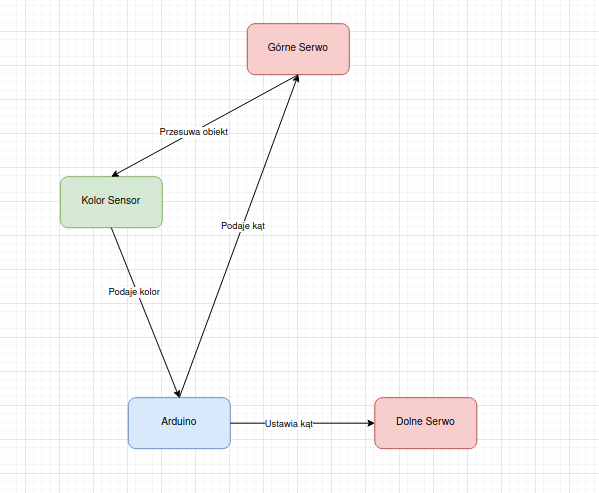
\includegraphics[scale=0.8]{wspol.png}
\subsubsection{Diagram interakcji}
\hspace{-1.75cm}%                
    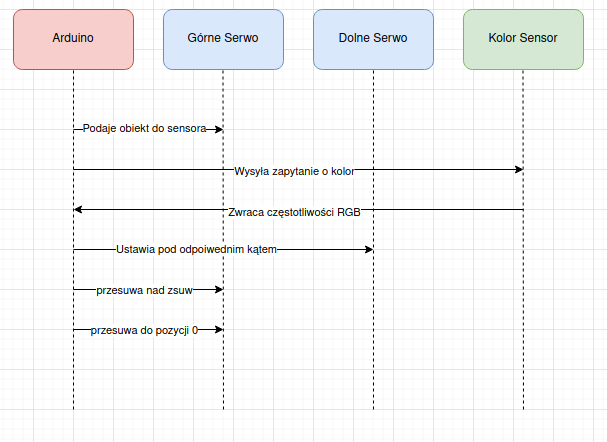
\includegraphics[scale=0.8]{inter.png}

\subsection{Diagram pinów(protokoły)}
\hspace{-1.75cm}%                
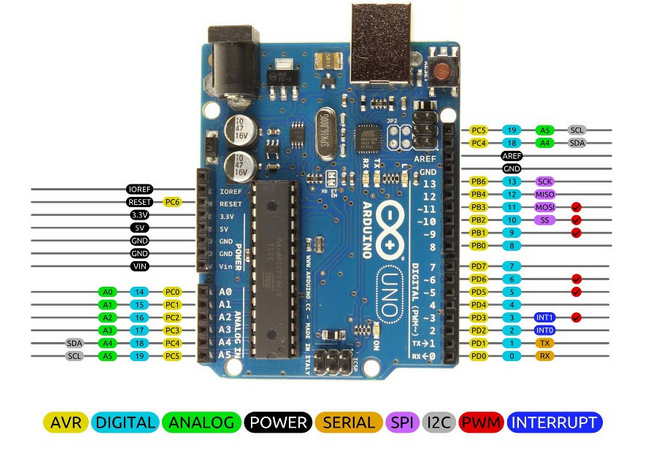
\includegraphics[scale=0.8]{protocol_ex.png}


\end{document}
